% Coding: utf-8
% Filename: aaai17_mage.tex
% Description: Paper submit to AAAI'17
% v0.0: File created. Motif-Aware Graph Embedding

% Standard settings by AAAI'17 authors' kit
\documentclass[letterpaper]{article}
\usepackage{aaai17}
\usepackage{times}
\usepackage{helvet}
\usepackage{courier}
\usepackage{graphics} % Using scalebox
\usepackage{graphicx} % Figures
\usepackage{dsfont} % Mathds
\usepackage{amsmath, amsthm, amssymb} % Align environment, definition (theorem)
\usepackage[ruled,vlined]{algorithm2e} % Use algorithm environment
\DeclareMathOperator*{\argmax}{arg\,max} % Objective argmax
\newtheorem{ntdef}{Definition}
\setlength{\pdfpagewidth}{8.5in}
\setlength{\pdfpageheight}{11in}
% PDF metadata
\pdfinfo{
    /Title (Motif-Aware Graph Embedding)
    /Author (Hoang Nguyen, Shun Nukui, Tsuyoshi Murata)
    /Keywords (Graph embedding, Latent representation, Complex network, Motif, Random walk, Biased random walk, MAGE)
}
% Section number
\setcounter{secnumdepth}{0}
% Title and authors
\title{Motif-Aware Graph Embedding}
\author{
    Anonymous Author(s) \\
    Anonymous Institute \\
    Anonymous Email Address(es) \\
}

%% Paper content
\begin{document}
    \maketitle

    \section{Abstract}
       Given a large complex graph, how can we have a lower dimension real-vector representations 
       of vertices that preserve structural information? Recent advancements in graph embedding 
       have adopted word embedding techniques and deep architectures to propose a feasible solution 
       to this question. However, most of these former researches consider the notion of ``neighborhood'' 
       by vertex adjacency only. In this paper, we propose a novel graph embedding algorithm that employs 
       motif structures into the latent vector representation learning process. Our algorithm learns 
       the graph latent representation by contrasting between different type of motif-biased random walk. 
       We showed that our algorithm yields more accurate embedding results compared to other existing 
       algorithms through various graph mining benchmark tasks.

    \setcounter{secnumdepth}{2}
    \section{Introduction}
        The graph (or network) data model is a useful tool for a wide range of disciplines, and
        it is essential to have a low dimensionality representation of a complex graph. In its
        simplest form, a graph is an ordered set of vertices connected by edges. Being simple
        and expressive, the graph-theoric approach has been applied in many scientific fields
        for untangling complex discrete structures. For example, the study conducted by 
        MP Van Den Heuvel suggested that the human brain functional network provides many new
        discoveries about our brain's organization \cite{BrainNetHeuvel}. The same approach
        for structural analysis can be found in other fields such as chemistry \cite{molecule}, 
        physics \cite{physicnet}, and sociology \cite{socialnet}. However, the graph analysis
        process often becomes intractable due to the complexity of the data. In such case,
        the graph usually contains several thousand to millions of vertices and edges.
        Therefore, it is desirable to have a compact latent representation of the graph while
        its statistical properties are retained. A \emph{high-quality} latent representation
        of a graph can benefit machine learning algorithms in many ways. For instance, 
        the result and runtime of machine algorithm will be improved thanks to the low
        dimensionality of the data. On the other hand, instead of relying only on graph 
        mining algorithms to analyze some given data, researchers can also apply other
        machine learning algorithms on the learned latent representation to make predictions.
        Conventionally, the latent representation learning procedure on a graph is called
        \emph{graph embedding}.

        % Include fig 1 dimensionality reduction task explaination here.
        \begin{figure}
            \centering
            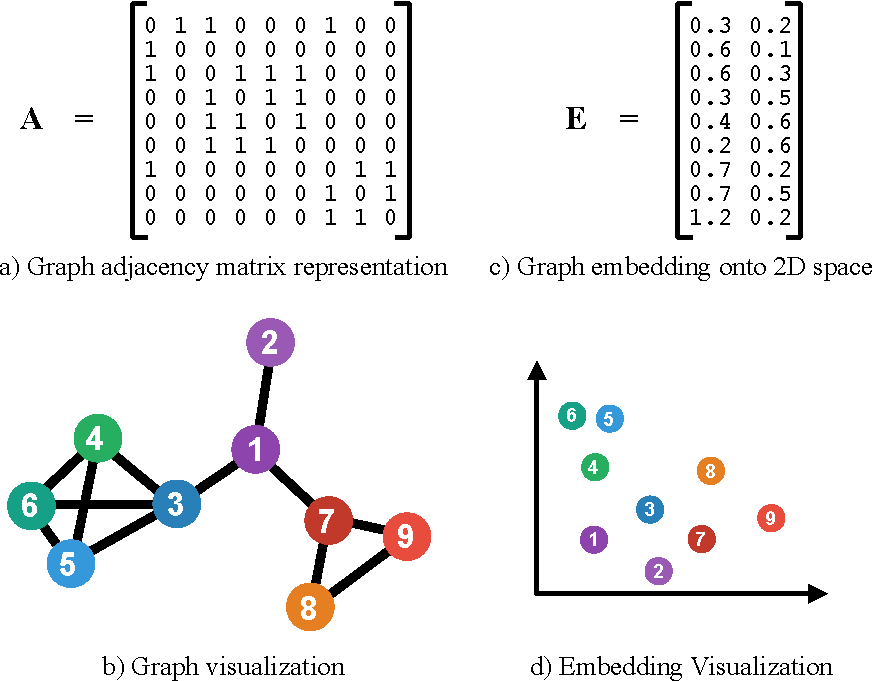
\includegraphics[width=0.45\textwidth]{fig1_dimrec}
            \caption{Graph dimension reduction.}
            \label{fig:dimrec}
        \end{figure}

        \emph{Learning} a high-quality latent representation is a challenging task. Traditionally,
        dimensionality reduction technique such as PCA \cite{pca}, CCA \cite{cca}, and IsoMap 
        \cite{isomap} are used. Although these aforementioned techniques have a profound theoretical
        background \cite{dimrecrev}, they are impractical due to computational drawbacks. To address
        the dimensionality problem, Peperozi et al.\ proposed Deepwalk - a Skipgram-based algorithm
        for graph embedding \cite{deepwalk}. Different from traditional linear algebra approach,
        Deepwalk learns the latent representation from the probabilistic point of view. By treating
        a random series of vertices as if it is a sentence of words, Deepwalk adopts the operation
        of Skipgram model \cite{skipgram} to learn a vertex's latent representation. Following
        Deepwalk, other Skipgram-based graph embedding algorithms which aim to improve embedding
        quality were proposed \cite{grarep, line, planetoid, node2vec}. However, these algorithms
        do not consider the intrinsic \emph{motif structure} of a graph. Therefore, the performance
        of these algorithms depends heavily on heuristic hyper-parameter tuning.

        % Include fig 2 sentence vs random walk.
        \begin{figure}
            \centering
            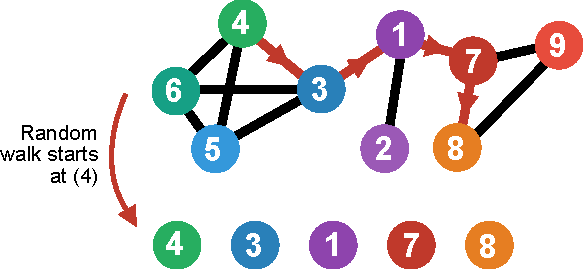
\includegraphics[width=0.4\textwidth]{fig2_congen}
            \caption{Random walk generates ``sentence'' from graph.}
            \label{fig:congen}
        \end{figure}

        In this work, we propose an algorithm which controls both graph context and negative samples
        generation. The motif-aware context generation aims to emphasize the importance of local
        motif community, which is a strong indicator for true community in a graph. On the other hand,
        negative sampling is known to be the state of the art technique to estimate the normalization
        factor of a probabilistic model. Instead of sampling from a distorted unigram distribution as
        suggested by Mikolov et al. \cite{skipgram}, we propose a motif-aware method to generate 
        negative samples from a graph. Generally, our algorithm, named Motif-Aware Graph Embedding (MAGE),
        has two following advantages:

        \begin{itemize}
            \setlength{\parskip}{0pt}
            \item Positive samples are generated using a motif-biased walk. This motif-aware context 
                generation procedure is backed by the hypothesis that vertices in the same motif
                are more likely to belong to the same community \cite{juremotif, harvardmotif}.
                By selecting the appropriate motif for each graph, we have a sensible way to control
                the context generated for embedding.
            \item Negative samples are also generated using a motif-biased walk. However, by choosing
                the \emph{opposing} motif to the characteristic motif of the graph, we have a concrete
                method to ``escape'' the motif community, which produces contrasting negative
                samples, hence better quality embedding.
        \end{itemize}

        Our algorithm is implemented on Keras \cite{keras} framework. The implementation and experimental
        results are available on Github. (TODO: ADD FOOTNOTE).

        The remaining of this paper is divided into 4 parts. Section 2 provides additional information
        about related work on graph embedding and graph motif. Section 3 presents our algorithm and
        experimental design. Section 4 and 5 discusses results and conclusion.

    \section{Related Works}
        \subsection{Skipgram Model}
            Representation learning has been one of the keys to the success of machine learning 
            algorithms \cite{bengioreprev}. In the context of natural language processing (NPL),
            representation learning becomes even more important as the data has a discrete, but
            high-dimension nature. To address the dimensionality problem in NLP, Mikolov et al.\ have
            proposed the Skipgram model \cite{skipgram}. Instead of maximizing the n-gram distribution
            as prior works, Skipgram maximizes the co-occurrence probability of context words given a
            target word. The softmax potential function for a context word given a target 
            word is given by:

            \begin{equation}
                \label{eq:model}
                \mbox{Pr} (v_c | v_t) = \frac{\exp{( \langle \omega_{v_c} ,  \omega_{v_t} \rangle )}}{\sum_{k \in V} \exp{( \langle \omega_{v_k} ,  \omega_{v_t} \rangle )}},
            \end{equation}
            
            \noindent
            where $ \langle \cdot ,  \cdot \rangle $ is vector dot product; $ v_c $ and $ v_t $ are the
            tokens for the context word and the target word respectively; $\omega_{v_t}$ is the embedding
            vector selected from the \emph{embedding matrix} by the token $v_t$; $\omega_{v_c}$ is the
            embedding vector selected from the \emph{context matrix} by the token $v_c$.

            Based on equation~\ref{eq:model}, the objective of Skipgram model is to maximize the following
            average log-likelihood:

            \begin{equation}
                \label{eq:avgloglikelihood}
                \mathcal{O} = \max \left( \frac{1}{T} \sum_{t=1}^{T} \sum_{-c \leq j \leq c, j \neq 0} \log \mbox{Pr} (v_{t+j} | v_t) \right)
            \end{equation}

            The intrinsic intractable problem for softmax model is normalization factor computation. 
            Therefore, the normalization factor in equation~\ref{eq:model} needs to be estimated by 
            approximation techniques such as Hierarchical Softmax \cite{hs} or Noise Contrastive estimation
            \cite{nce}. In their landmark paper, Mikolov et al.\  also proposed \emph{Negative Sampling} - a 
            simplified version of noise contrastive estimation \cite{skipgram}. The log-likelihood of 
            under negative sampling scheme is given by:

            \begin{equation}
                \label{eq:objneg}
                \begin{aligned}
                \log \mbox{Pr} (v_c | v_t) & = \log \sigma( \langle \omega^{\scalebox{0.7}{nce}}_{v_c} , \omega^{\scalebox{0.7}{emb}}_{v_t} \rangle ) \\
                + \sum_{i=1}^{k} & \mathds{E}_{\omega_{v_i} \sim P_n(\omega)} \left[ \log \sigma( -\langle \omega^{\scalebox{0.7}{nce}}_{v_i} , \omega^{\scalebox{0.7}{emb}}_{v_t} \rangle) \right],
                \end{aligned}
            \end{equation}
            
            \noindent
            where $\sigma$ is the sigmoid function; $\omega_{v_i}$ is sampled from the user-defined
            negative distribution $P_n(\omega)$; $k$ is the number of the negative samples for each target
            $v_t$; $\omega^{\scalebox{0.7}{nce}}_{v_c}$ and $\omega^{\scalebox{0.7}{emb}}_{v_t}$ 
            represent embedding vectors for words $v_c$ and $v_t$ respectively. Notice that the
            context embedding matrix (named ``nce'') and the target embedding matrix (named ``emb'')
            are different.

            Similar to Noice Contrastive Estimation, Negative Sampling changes log-likelihood
            maximization objective to positive/negative samples classification task. As discussed
            in depth by Gutmann et al.\ and Mikolov et al.\ , the choice of negative distribution 
            $P_n(\omega)$ can greatly affect the quality of the embedding result. Therefore, an
            appropriate negative sampling setting will benefit the system in term of statistical
            performance and computational cost.

        \subsection{Graph Embedding}
            
            Inspired by the power-law similarity between the vertex frequency distribution in
            random walks and the word frequency distribution of English text, Peperozi et al.\ proposed
            Deepwalk algorithm to \emph{learn} the latent representations of vertices in a
            graph \cite{deepwalk}. The operation of Deepwalk is based on hierarchial-softmax
            Skipgram, the only different is artificial ``sentences'' are generated by performing
            random walk on the graph. Inheriting the advantages of the Skipgram model, Deepwalk
            has been successful in various graph-related machine learning tasks. However, the weakness
            of Deepwalk is in the fact that it ignores the graph's deep structures which cannot 
            be discovered only by random walks. 

            % Figure for structure-aware context generation (LINE)
            \begin{figure}
                \centering
                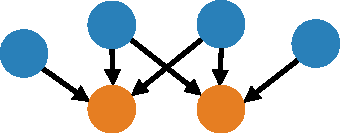
\includegraphics[width=0.3\textwidth]{fig3_line}
                \caption{LINE generates context where blue vertices are together, whereas random walk cannot. It is trivial to see the bipartite structure in this figure.}
                \label{fig:line}
            \end{figure}

            In one of the researches subsequent to Deepwalk, Tang et al.\ hinted the advantages 
            of structure-aware graph context generation in their citation network experimental 
            results \cite{line}. In their work, Tang et al.\ proposed LINE, which consider the
            second-order proximity into the embedding process. By constructing half the embedding
            vector with Deepwalk, and the other half with vertices that have second-order proximity,
            LINE has improved embedding results compare to Deepwalk. However, in the most recent
            graph embedding research, Grover et al.\ reported some unexpected poor performance
            from LINE in friendship-based graphs \cite{node2vec}. On the contrary, we noticed that 
            LINE has exceptionally good performance in some graphs that have acyclic structure 
            (e.g.\ citation networks). We also found the similarity between the definition of 
            second-order proximity in \cite{line} and the bipartite motif (Figure~\ref{fig:motifs}).
            From the observations above, we hypothesize that the graph embedding quality can be
            improved by taking advantage of the statistically significant motifs with the graph.

            % Figure for node2vec vs node community
            \begin{figure}
                \centering
                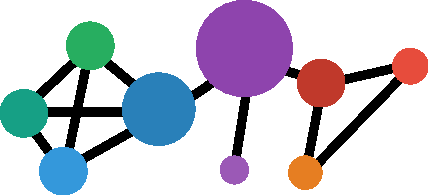
\includegraphics[width=0.3\textwidth]{fig4_n2v}
                \caption{Node2vec emphasizes central ``important'' vertices.}
                \label{fig:n2v}
            \end{figure}

            In 2016, Grover et al.\ proposed \emph{node2vec}, an algorithm based on biased random
            walks. This idea of using biased random walk to manipulate graph context generation
            is aligned perfectly with our idea. However, while node2vec aims to emphasize statistically
            important \emph{vertices}, our algorithm aims to emphasize the local motif community
            structure. Another noteworthy graph embedding research is Planetoid \cite{planetoid} 
            proposed in 2015 by Yang et al. While other graph embedding algorithms is unsupervised, 
            Planetoid is a semi-supervised approach. In addition to random walk graph context generation, 
            Planetoid generates another context using the training community labels. Due to the
            semi-supervised learning procedure of Planetoid, we consider it belongs to another
            category of algorithm. However, we will discuss the integration of Planetoid to our
            algorithm in later section.

        \subsection{Network Motifs}

            Network motifs are defined to be recurring and regulating patterns in a complex network 
            \cite{netmotif}. First mentioned by Milo et al. \cite{motifblockmilo}, network motifs
            soon became a topic of attention in many research fields especially in biology and sociology
            \cite{masoudirev}. Recent researches suggested that network motifs withhold the structural 
            information of the network \cite{juremotif, harvardmotif, deepgraphkernel}. Due to the
            computational complexity of graph isomorphism, in most researches, the studied motifs 
            often has a small size (number of vertices in a motif is less than 4) \cite{motifdecrev}.
            Figure~\ref{fig:motifs} presents some of the most noteworthy motifs.

            % Figure for motifs - 2 columns. On page 3. (TODO: DRAW FIGURE)

            % Formal motif definition.
            \begin{ntdef}
                \textbf{Network motif} are patterns of interconnections that recur in many different
                parts of a network at frequencies much higher than those found in randomized networks
                \cite{motifblockmilo}.
            \end{ntdef}

            The sentence ``a friend of a friend is a friend'' makes sense to us in real life. Interestingly,
            from the graph-theoric point of view, social networks exhibit the similar rule of relationship.
            In the study conducted by Katherine Faust, the author compared the social interaction 
            networks of animals using the triangle motif \cite{comsocialnetwork}. Faust pointed
            out the representation power of different directed triangle motifs to each type of animal social
            interaction, and also suggested that triangle motifs play a central role in a social network's
            structure. Moreover, studying the Stanford's SNAP network datasets archive \cite{SNAP}, 
            we also observe that the social networks have higher triangle count compared to other type of 
            network such as citation network. In conclusion, although there has not been a concrete proof 
            for the importance of network motifs in a complex network, we cannot ignore the pragmatic 
            representation capability of network motifs.

    \section{Method}

        In this section, we present our algorithm in detail. Although there are many different types of motif
        in a graph, within this paper, we only consider undirected triangle motif (figure~\ref{fig:motifs}),
        undirected wedge motif (figure~\ref{fig:motifs}), and undirected bipartite motif 
        (figure~\ref{fig:motifs}) for the sake of simplicity. Other types of motif and directed graph
        extension is discussed in Section 5.

        \begin{figure}
            \centering
            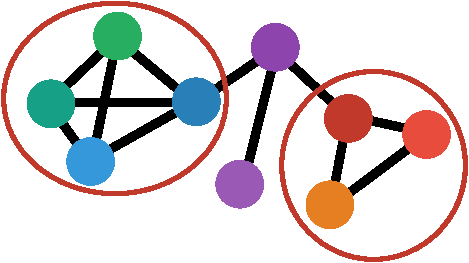
\includegraphics[width=0.3\textwidth]{fig5_mage}
            \caption{MAGE discovers local motif structure.}
            \label{fig:n2v}
        \end{figure}

        \subsection{Motif-Aware Context Generation}

            Our algorithm is based on the Negative Sampling Skipgram model (NEG-Skipgram) \cite{skipgram}.
            As mentioned in the previous section, Skipgram-based graph embedding \emph{is} word embedding,
            the difference is the ``sentences'' are generated by a random process in graph embedding.
            We first discuss the graph context generation phase, also called the positive sample generation.
            In order to highlight the local motif structure given a target vertex, we define a motif-biased
            random walk (or \emph{motif walk} for short). Our motif walk can be viewed as a Monte Carlo
            Markov Chain \cite{mcmc}, whose number of states equals the motif size. At each step along 
            the motif walk, an adjacent vertex is chosen by the rejection sampling procedure. The rejection
            probability depends on the pre-defined states of the Markov Chain. Algorithm~\ref{al:amotif} 
            describes the motif walk for an arbitary motif.

            \begin{ntdef}
                Monte Carlo Markov Chain is awesome. (TODO: FILL THIS)
            \end{ntdef}

            % Figure for triangle MCMC


            \begin{algorithm}
                \DontPrintSemicolon
                \KwData{Undirected Graph $G = (V, E)$;}
                \KwIn{length, MCMC chain}
                \KwResult{List containing vertices in the motif walk;}
                initialization\;
                \While{Not full yet} {
                    Walk around\;
                    \eIf{walk fail} {
                        walk again\;
                    } {
                        continue to walk\;
                    }
                }
                \caption{Motif walk based of MCMC (TODO: FILL THIS)}
                \label{al:amotif}
            \end{algorithm}

            The motif statistic of a graph is the key input to our algorithm. As mentioned by Tran et al.\ in
            their research on motif detection algorithms, motif detection is a costly operation. The
            exact motif statistic is desiable, but costly to obtain. However, we found that only one or 
            two most characteristic motifs are enough to improve the graph embedding quality. Therefore, 
            to keep the topic of the paper focused, we pose an assumption that we know in advance the most
            statistically significant motif for a given graph. 

        \subsection{Negative Sampling}

            For each defined motif walk in the previous section, it is trival to define the inverse version
            of it. For example, the inverse of the aforementioned triangle motif walk is the wedge motif
            walk (figure~\ref{fig:motifs}). In addition to the traditional unigram-distribution negative
            sampling, we further emphasize the importance of motif structure by sampling negative samples
            from the corresponding inverse version of the motif walk that generated graph context. 
            Figure~\ref{fig:mneg} illustrates our reason for motif-aware negative sampling.

            % Figure for negative motif sampling.

        \subsection{MAGE: Motif-Aware Graph Embedding}

            \begin{algorithm}
                \DontPrintSemicolon
                \KwData{Undirected Graph $G = (V, E)$;}
                \KwIn{length, MCMC chain}
                \KwResult{List containing vertices in the motif walk;}
                initialization\;
                \While{Not full yet} {
                    Walk around\;
                    \eIf{walk fail} {
                        walk again\;
                    } {
                        continue to walk\;
                    }
                }
                \caption{MAGE}
                \label{al:mage}
            \end{algorithm}

            Figure~\ref{fig:mage} and algorithm~\ref{al:mage} illustrate our MAGE algorithm. In summary, 
            there are 4 context generation operations: two of them are positive sampling, and the other
            two are negative sampling. To control the number of samples for each type, we introduce a 
            hyper-parameter $\alpha$. For example, assume that MAGE generates 6 positve samples and 
            20 negative samples for each target vertex, with $\alpha=0.5$, MAGE yeilds 3 postive samples 
            from motif walk, 3 postive samples from random walk, 10 negative samples from vertex unigram
            distribution, and 10 negative samples from inverse motif walk.  Finally, we define the 
            objective function as follow:

            % Figure for the deep learning framework.

            \begin{equation}
                \label{eq:mageobj}
                \mathcal{L} = (1-\alpha) \mathcal{L}_{\scalebox{0.7}{random}} + 
                                \alpha \mathcal{L}_{\scalebox{0.7}{motif}} ,
            \end{equation}

            \noindent
            where $\mathcal{L}_{\scalebox{0.7}{random}}$ is given in equation~\ref{eq:objneg};
            $\mathcal{L}_{\scalebox{0.7}{motif}}$ is defined as:

            \begin{equation}
                \label{eq:objmotif}
                \begin{aligned}
                    \log \mbox{Pr} (v_c | v_t) & = \mathds{E}_{\omega_{v_c} \sim P_m(\omega)} \left[ \log \sigma( \langle \omega^{\scalebox{0.7}{nce}}_{v_c} , \omega^{\scalebox{0.7}{emb}}_{v_t} \rangle ) \right] \\
                + \sum_{i=1}^{k} & \mathds{E}_{\omega_{v_i} \sim (1-P_m(\omega))} \left[ \log \sigma( -\langle \omega^{\scalebox{0.7}{nce}}_{v_i} , \omega^{\scalebox{0.7}{emb}}_{v_t} \rangle) \right],
                \end{aligned}
            \end{equation}

        \subsection{Learning framework}
            
            Up to this point of the paper, we have presented the graph context generation procedures.
            In this section, we present the neural network implemented on Keras \cite{keras} 
            (with Theano \cite{theano} backend). One advantage of our implementation is that
            it can run on both CPU and GPU (when available) thanks to the Keras wrapper. Our
            neural network contains 3 modules. Firstly, there are two embedding matrices of 
            the same shape (\texttt{num\_vertices}, \texttt{emb\_dim}). The matrix named ``emb''
            contains embedding vectors for the target vertices, while the other matrix named
            ``nce'' contains embedding vectors for the context vertices. Secondly, the computation
            module computes the dot product of each samples in the mini-batch, applies the
            sigmoid function, then yeilds the final logit. The last modules compute the
            the cross-entropy \cite{xentropy} of samples in the mini-batch and its positive/negative
            labels. Figure~\ref{fig:mage} present the block diagram of our learning framework.
            To optimize the binary cross entropy objective, we use Adam \cite{adam} as the 
            mini-batch gradient optimizer.
            
    \section{Experiments and Result}

        \subsection{Experiments design}
            
            In our experiments, we compare our approach (MAGE) with Deepwalk \cite{deepwalk}, 
            LINE \cite{line}, and node2vec \cite{node2vec} by multilabel classification. 
            Table~\ref{tb:data} gives graph statistics and its corresponding machine learning task. 

            \begin{table}
                \centering
                \resizebox{\columnwidth}{!}{%
                    \begin{tabular}{c r r r}
                        \textsc{Dataset} & \textsc{\#Classes} & \textsc{\#Vertices} & \textsc{\#Edges} \\
                        \hline \\
                        \textsc{BlogCatalog} & 39 & 10,312 & 333,983 \\
                        \textsc{Wikipedia} & 40 & 4,777 & 184,812 \\
                        \textsc{Citeseer} & 6 & 3,327 & 4,732 \\
                        \textsc{Youtube} & 47 & 1,138,499 & 2,990,443 \\ 
                        \end{tabular}%
                }
                \label{tb:data}
                \caption{Dataset statistics}
            \end{table}

            Blogcatalog \cite{blogcatalog} is a social network of bloggers. The labels represent
            a blogger's interest. There are 39 labels in total, each blogger (vertex) has at least
            one label. Since Blogcatalog is a social network, we chose undirected triangle motif
            walk for this graph. On the other hand, Wikipedia \cite{wiki} and Citeseer \cite{citeseer} 
            are coocurrence and citation networks. Therefore, we employ bipartite motif for 
            these networks. The last graph we consider is Youtube, which is especially
            large with more than 1 million vertices. Since Youtube is also a friendship network,
            we also use triangle motif in context generation.

            Conventionally, multilabel classification task is contructed as Peperozi et al.\ suggested
            in their paper. The embedding vector for each vertex will be treated as the feature
            vector for a One-versus-Rest logistic regression with L2 regularizaation. We split the 
            data into training set and testing set. The result reported here is the weighted f1-macro and
            f1-micro score with split ratio of 0.5. One exception is with the Youtube network, the
            split ratio is 0.1 (training data : testing data) due to the size of the network.

            In all of our experiments, we use the same hyper-parameters which gave the best
            reported results in previous researches. For our algorithm, the hyper-parameters
            are given in table~\ref{tb:hyper}.


            \begin{table}
                \centering
                \resizebox{\columnwidth}{!}{%
                    \begin{tabular}{c r r }
                        \textsc{Hyper Parameter} & \textsc{Abbr.} & \textsc{Value} \\
                        \hline \\
                        Embedding dimenison & \texttt{emb\_dim} & 128 (Youtube=8) \\
                        Skip window size & \texttt{window\_size} & 10 \\
                        Walk length & \texttt{walk\_length} & 80 \\
                        \#Negative samples & \texttt{neg\_samp} & 30 \\ 
                        \#Positive samples & \texttt{num\_skip} & 5 \\
                        \#Motif weight & $\alpha$ & 0.2 \\
                        \#Motif bias & $\beta$ & 0.9 \\
                        \end{tabular}%
                }
                \label{tb:hyper}
                \caption{MAGE Hyper-parameters}
            \end{table}

        \subsection{Experimental Results}

            Experimental results are presented in table~\ref{tb:result}.

            \begin{table}
                \centering
                \resizebox{\columnwidth}{!}{%
                    \begin{tabular}{c | c | c | c | c}
                        \textbf{\textsc{Method}} & \textsc{BlogCatalog} & \textsc{Wikipedia} & \textsc{Citeseer} & \textsc{Youtube} \\
                        \hline
                        & & & &  \\
                        Spectral clustering & 0.28 * & 0.1 & 0.1 & 0.1  \\
                        Deepwalk & 0.20 & 0.1 & 0.1 & 0.1 \\
                        LINE & 0.07 & 0.1 & 0.1 & 0.1 \\
                        Node2Vec & 0.11 & 0.25 & 0.1 & 0.1 \\
                        \textbf{MAGE} & 0.24 & 0.1 & 0.1 & 0.1 \\
                        \end{tabular}%
                }
                \label{tb:result}
                \caption{Multilabel classification weighted f1-macro}
            \end{table}

    \section{Discussion}

            The Skipgram model proposed by Mikolov et al. \cite{skipgram} is a powerful model 
            in natural language processing. Under the Distributional Hypothesis \cite{disthyp},
            the Skipgram model maximizes the occurent probability of context words given a target
            word. 

\end{document}
